\documentclass{beamer}
\usetheme{CWRU}

\title{Exploring Alternative Routes Using Multipath TCP}
\author{Stephen Brennan}
\institute{Case Western Reserve University}
\date{June 5, 2017}

\usepackage{appendixnumberbeamer}
\usepackage{pgfpages}
\usepackage{wrapfig}
\usepackage[export]{adjustbox}
\usepackage{graphicx}
\usepackage{fancyvrb}
\setbeamertemplate{note page}[plain]
\setbeameroption{show notes on second screen=right}
\setbeamertemplate{navigation symbols}{}%remove navigation symbols
\AtBeginNote{%
    \let\enumerate\itemize%
    \let\endenumerate\enditemize%
}

\newcommand{\FigureSlide}[2]{
  \begin{frame}[plain]
    \begin{centering}
      \vfill
      \includegraphics[max width=\textwidth,max height=\textheight]{#1}
      \vfill
      \end{centering}
    \note{#2}
  \end{frame}
}

\newcommand{\SectionHead}[2]{
  \begin{frame}{#1}
    \tableofcontents[currentsection,hideallsubsections]
    \note{#2}
  \end{frame}
}

\begin{document}
\frame{
  \titlepage
  \note{
    Hello everyone. I'm Stephen, and today I'll be discussing my thesis,
    entitled ``Exploring Alternative Routes Using Multipath TCP''.
  }
}

\section{Introduction}

\begin{frame}{Overview}
  \tableofcontents[hideallsubsections]
  \note{
    Here is how this talk is going to be structured. First, I'll be giving a bit
    of motivation for this project, along with a problem statement and our
    background information. Next, I'll discuss related work in this field, and
    show how this thesis fits into the current research. After that, I'll give
    an overview of the implementation of the components of the thesis. Next,
    I'll discuss the experiments I used to validate the mechanism, and finally
    we'll conclude with a brief summary and discussion of future work.
  }
\end{frame}

\FigureSlide{figures/InternetSlide.pdf}{
  Okay, so let's get started! I want to start off with a brief and simplified
  look at the Internet. As we know, the Internet is made up of routers, the blue
  dots, and Autonomous Systems, the tan groups. The task of each router is to
  forward small packets of information toward their final destination. The route
  that packets take is determined by a lot of factors.

  While this project isn't directly about routing, let's discuss some of these
  factors. Routing is typically performed, in some way or another, by an
  application of Dijkstra's algorithm for finding a shortest path. While this
  might be optimal in a theoretical sense, the practical application is not, and
  for several reasons.

  For one, routing algorithms are going to work by ``hop count'',
  meaning that a shorter path should be preferred, even if the longer path might
  actually exhibit better properties. For another, the Autonomous Systems are
  frequently businesses or ISPs, and the connections they make are determined by
  business agreements. They may create policies that are less than optimal in
  order to fulfill business objectives.
}

\begin{frame}
  \frametitle{Internet Routing Inefficiencies}
  \begin{columns}
  \begin{column}{0.7\textwidth}
  \begin{itemize}
  \item The default route is not always the best, in terms of latency or
    reliability
  \item Peering agreements and policy based routing can result in suboptimal
    routing decisions \cite{detour}
  \item A route that passes through a ``detour'' may be better
  \end{itemize}
  \end{column}
  \begin{column}{0.3\textwidth}
    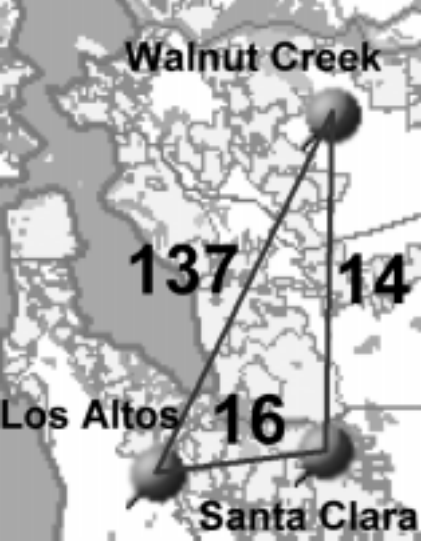
\includegraphics[width=\textwidth]{figures/detour.png} \\
    \textit{Figure from \cite{detour}}
  \end{column}
  \end{columns}
  \note{
    Research in the field has been able to fairly concretely demonstrate the
    problem. Just because your traffic takes a particular route, doesn't mean it
    is going to be the best path for you, in terms of latency or reliability.

    Instead, if you were to route your packets to a ``detour'' and then to the
    final destination, you might actually get path which has better round trip
    time or loss rate. On the right we have an example of a situation found by a
    study, where the default route from Los Altos to Walnut Creek had a round
    trip time of 137 ms, while the combined round trip time of a path via Santa
    Clara was only 30 ms. The reason was that the default route actually
    traveled through Chicago!
  }
\end{frame}

\FigureSlide{figures/detour-packetloss.png}{
  This effect is not limited to isolated examples, either. This same study
  looked at a large group of computers on university networks. They computed
  latency and packet loss rates between each pair of computers. Then, they
  searched for pairs in which the ``triangle inequality'' was violated.

  This graph shows packet loss rates between pairs of computers. The blue is the
  default Internet routed path, and the yellow is the best alternative path that
  uses a single detour. Most of the yellow dots are actually on the zero line.

  You can see here that for a large majority of pairs, there is an alternative
  route that is more reliable. For a small fraction here, the difference in
  reliability is actually huge.
}

\begin{frame}
  \frametitle{Access Link Underutilization}

  \begin{itemize}
  \item Fiber-to-the-home is coming!
  \item However, residential bandwidth is not fully utilized
    \cite{fibertothehome}
    \begin{itemize}
    \item Short-lived TCP sessions?
    \item Small TCP initial window?
    \item Network core can't support bandwidth?
    \end{itemize}
  \item Using alternative routes can improve performance
  \item Aggregating multiple routes can perform even better
  \end{itemize}

  \note{
    Now let's take a brief detour and discuss something else. Recently, we've
    been seeing some exciting trends in residential bandwidth. New access links
    are always being created, and the latest improvement is fiber to the home.
    These can provide up to Gigabit speeds to a home network. However, we've
    had studies right here at CWRU showing that these residential links don't
    use most of that capacity.

    There are several good explanations for this. Short lived TCP sessions may
    never leave the slow-start stage. A small TCP initial window will limit the
    throughput that can be achieved in a reasonable amount of time. But there's
    also the possibility that the network core is becoming the bottleneck for
    some of these connections.

    Two things seem to follow. First, there are good chances that a detour route
    could provide better throughput for a TCP connection, as studies have
    already demonstrated. Second, if we have extra access link capacity, why not
    use these paths in combination with each other, rather than choosing only
    one?
  }
\end{frame}

\begin{frame}
  \frametitle{Contributions}

  \textbf{Problem:} Internet routing inefficiencies can prevent TCP connections
  from achieving their full potential throughput.

  \vspace{0.5cm}

  \textbf{Solution:} A system which can use and aggregate alternative routes for
  TCP connections.

  \vspace{0.5cm}

  \textbf{Contributions:}

  \begin{itemize}
  \item A mechanism for adding alternative routes to Multipath TCP (MPTCP)
    sessions among single-homed hosts.
  \item An evaluation of this mechanism on emulated and real-world networks.
  \end{itemize}
  \note{
    Putting this together, we have a problem: routing inefficiencies can prevent
    TCP connections from achieving their full potential throughput. Access links
    may be capable of much better bandwidth than a user actually gets.

    Our solution is to create a system which can use and aggregate alternative
    paths for TCP connections. Using these paths means that it can route traffic
    along them. Aggregation means combining the potential throughput of both
    paths, to get better throughput than either.

    The contributions this thesis makes are twofold: first, a mechanism that
    allows single-homed devices to add subflows along alternative routes via
    MPTCP. Second, an evaluation of this system on emulated and real world
    networks.
  }
\end{frame}

\section{Background}
\SectionHead{}{}
\subsection{Multipath TCP}

\begin{frame}
  \frametitle{Multipath TCP}

  \begin{itemize}
  \item Multi-homed devices are becoming more common
    \begin{itemize}
    \item Smartphones
    \item Datacenters
    \item Laptops
    \end{itemize}
  \item TCP still views a connection as a five-tuple: (TCP, Source IP, Source
    port, Destination IP, Destination Port)
  \item Multi-homed devices are forced to choose a network interface
  \item Multipath TCP is an extension to TCP, allowing hosts to use multiple
    addresses in the same connection
  \end{itemize}
    \note{

      This project is based on MPTCP. While it's not my intent to give a
      comprehensive protocol description in this presentation, I do want to give
      enough background to understand how my project uses it.

      Recently, we've seen a rise in devices that have multiple ways to connect
      to the Internet, network interfaces. For instance, smartphones include
      cellular and WiFi radios, and can be connected to the Internet on both.
      Recent data centers have been taking advantage of multiple interfaces and
      highly redundant network topologies. Laptops can also contain WiFi,
      Ethernet, and even cellular radios.

      Unfortunately, TCP was designed for a simpler time, when computers had a
      single interface and their addresses never changed. This forces
      multi-homed devices to decide which interface they'll use and stick to
      that choice.

      Multipath TCP aims to solve this problem. It is an extension to TCP (not a
      replacement) that allows devices to make use of all of their network
      interfaces and addresses in a single connection.
    }
\end{frame}

\begin{frame}{Design Goals}

  \begin{itemize}
  \item Improve performance and reliability over current TCP, by aggregating
    paths created by multiple interfaces.
  \item Do no harm to single-path TCP, by taking no more bandwidth over shared
    bottlenecks than standard TCP would
  \item Remain compatible with TCP applications and the Internet
    \begin{itemize}
    \item Present the same socket API to applications
    \item Remain similar to TCP on the wire, to remain compatible with Internet
      middleboxes
    \end{itemize}
  \end{itemize}
  \note{
    As a protocol, MPTCP has a few key design goals. First, it is designed to
    improve performance and reliability compared to standard TCP. Second, it
    should not do any harm to existing single-path TCP. Third, it should remain
    compatible to applications and to the Internet as a whole.
  }
\end{frame}

\begin{frame}[fragile]
  \frametitle{Architecture}
  \begin{center}
\begin{BVerbatim}
                     +-------------------------------+
                     |           Application         |
+---------------+    +-------------------------------+
|  Application  |    |             MPTCP             |
+---------------+    + - - - - - - - + - - - - - - - +
|      TCP      |    | Subflow (TCP) | Subflow (TCP) |
+---------------+    +-------------------------------+
|      IP       |    |       IP      |      IP       |
+---------------+    +-------------------------------+
\end{BVerbatim}
  \end{center}
  \note{
    The way that MPTCP achieves this is by layering the protocol extension in
    between TCP and the application layer. An MPTCP connection consists of one
    or more (well, potentially zero or more) TCP connections, which we refer to
    as ``subflows''. These subflows bear some extra TCP options which provide
    signaling information, but other than that they behave very similarly to
    standard TCP. The only major difference is that their receive window is
    shared, rather than per-subflow. The MPTCP connection has its own sequence
    numbers, and each subflow has independent sequence numbers as well.
  }
\end{frame}

\begin{frame}
  \frametitle{Path Management}

  \begin{itemize}
  \item Subflows are established with a three way handshake
  \item First subflow uses \texttt{MP\_CAPABLE} option
  \item Subsequent subflows use \texttt{MP\_JOIN} option
  \item Additional addresses may be advertised using \texttt{ADD\_ADDR} at any
    time
  \item Either side may create new subflows at any time
  \end{itemize}
  \note{

    When we create an MPTCP connection, a three-way handshake occurs, just like
    standard TCP. However, the three-way handshake includes the MP CAPABLE
    option, signalling to the other host that it supports MPTCP. A SYNACK with
    MP CAPABLE signals that the passive opener supports MPTCP as well, and the
    final ACK with MP CAPABLE confirms the use of MPTCP. The contents of these
    options are key material, which is used to authenticate creation of new
    subflows.

    Subsequent subflows are created with a similar procedure, but using the MP
    JOIN option. The contents of the option this time are HMAC signatures based
    on the key material. If the HMAC can be verified, the hosts can be certain
    that they are communicating with the same host they initially established a
    connection with.

    An MPTCP implementation may advertise that it has additional addresses (and
    therefore additional interfaces) via an ADD ADDR option. There is also
    support for deletion.

    Finally, the MPTCP specification says nothing about when subflows should be
    created or destroyed. This is entirely left up to local policy, and of
    course research. In the Linux kernel implementation of MPTCP, a module
    interface exists for this, called the path manager.

  }
\end{frame}

\FigureSlide{figures/DataScheduling.pdf}{

  So, now that we have subflows, what do we do with them? How do we get data
  through them to the other application? Well, we do this with two important
  concepts: a data scheduler and the data sequence mapping.

  Imagine one host wants to send some data. It passes it through the send system
  call, and eventually the MPTCP stack has a large piece of data. A component
  called the scheduler gets to make the executive decision of how to divide up
  the data. It does this however it pleases, and the chunks make their way down
  to the subflows.

  In order to be able to put them back together, a data sequence signal is sent
  on the subflow.

}

\section{Related Work}
\SectionHead{}{
  Would love to discuss more, but limited time
}

\subsection{Overlay Networks}

\begin{frame}
  \frametitle{Resilient Overlay Networks}

  \begin{itemize}
  \item Rather than use only one detour, create an overlay network
  \item Overlay nodes use the Internet as their ``link layer''
    \note[item]{In Intro, discussed Detour study. RON is something of a
      spiritual successor. Rather than simple detours, use overlay networks.}
  \item Routing performed at each node using measured link characteristics
    \note[item]{Each node is an Internet host. Constantly monitoring link
      characteristics of network, updating routing tables with performance
      metrics.}
  \item Several studies based on RON:
    \note[item]{RON achieved good results, was testbed for additional studies.}
    \begin{itemize}
    \item Redundant multipath routing
      \note[item]{One study compared two routing strategies: adaptively choosing
      the best path, or redundantly using multiple paths. No aggregation.}
  \item ``Biologically inspired'' multipath routing
    \note[item]{Another - biologically inspired. Choose strongest path as
      primary, have several backups, involves differential equations and
      randomness.}
  \item mTCP \note[item]{mTCP: most important. A modification of TCP before
      MPTCP existed. Built on RON + userspace TCP stack. Did not have MPTCP
      compatibility concerns - routed segments across different paths. Worked on
      single-homed devices due to RON}
    \end{itemize}
  \end{itemize}
\end{frame}

\begin{frame}
  \frametitle{Other Related Items}

  \note[item]{Outside of overlay networks, several related pieces of work, both
    in research and in the standards bodies.}

  \begin{itemize}
  \item Source routing (IPv4) and segment routing (IPv6)
    \note[item]{Notable - it is possible to specify intermediaries in both IPv4
      and IPv6. For security reasons these aren't respected. Standards exist
      mainly for use in internal networks.}
  \item Binder: aggregating bandwidth of several Internet gateways
    \note[item]{One use of MPTCP that is very similar was called Binder. A rural
      town was away from any ISP. Had several potential gateways far away, but
      low bandwidth and not good reliability. Established connections across
      each gateway, and created an OpenVPN connection to an Internet-side
      server, with subflow across each.}
  \item SOSR: Scalable One-hop Source Routing \note[item]{Work inspired by RON,
      but trying to simplify. This work simply tunneled connections across a
      single hop, using a NAT approach similar to ours. Found they got most of
      RON's benefit without the full overlay system.}
  \item IETF MPTCP proxying draft
    \note[item]{Similar because allows single-homed devices to use MPTCP.
      However this approach expects non MPTCP server, and is ``transparent''
      proxy.}
  \end{itemize}
\end{frame}

\section{Implementation}
\section{Evaluation}
\section{Conclusion}

\appendix % slide numbering includes nothing after here

\section{References}
\begin{frame}[allowframebreaks]
  \frametitle{References}
  \bibliographystyle{ieeetr}
  \bibliography{paper.bib}
\end{frame}

\end{document}